% Research Paper for GECCO 2015
% by Nic McPhee, Kirbie Dramdahl, and David Donatucci

\documentclass{sig-alternate}

\usepackage{parskip}
\usepackage{times} %For typeface
\usepackage{graphicx}
\usepackage{algorithm}
\usepackage{algorithm,algorithmic}
\usepackage[justification=centering]{caption}[2007/12/23]
\usepackage{url}
\sloppy

\newcommand{\citep}[1]{\cite{#1}}

\DeclareGraphicsRule{.tif}{png}{.png}{`convert #1 `dirname #1`/`basename #1 .tif`.png}

\begin{document}

\conferenceinfo{GECCO'15,} {July 11-15, 2015, Madrid, Spain.}
\CopyrightYear{2015}
\crdata{TBA}
\clubpenalty=10000
\widowpenalty = 10000
    
\title{Impact of Crossover Bias in Genetic Programming}

\numberofauthors{1}
\author{
\alignauthor
Nicholas Freitag McPhee, M. Kirbie Dramdahl, David Donatucci\\
	\affaddr{Division of Science and Mathematics}\\
	\affaddr{University of Minnesota, Morris}\\
	\affaddr{Morris, MN USA-56267}\\
	\email{\{mcphee, dramd002, donat056\}@morris.umn.edu}
}

% This is more like how it "should" be done, but I think the previous approach might look nicer. They
% may force us to change it, though, to make it easier to scrape information.

%\numberofauthors{3}
%\author{
%\alignauthor
%Nicholas Freitag McPhee\\
%	\affaddr{Division of Science and Mathematics}\\
%	\affaddr{University of Minnesota, Morris}\\
%	\affaddr{Morris, MN USA-56267}\\
%	\email{mcphee@morris.umn.edu}
%\alignauthor
%M. Kirbie Dramdahl\\
%	\affaddr{Division of Science and Mathematics}\\
%	\affaddr{University of Minnesota, Morris}\\
%	\affaddr{Morris, MN USA-56267}\\
%	\email{dramd002@morris.umn.edu}
%\alignauthor
%David Donatucci\\
%	\affaddr{Division of Science and Mathematics}\\
%	\affaddr{University of Minnesota, Morris}\\
%	\affaddr{Morris, MN USA-56267}\\
%	\email{donat056@morris.umn.edu}
%}

\date{} 
    
\maketitle

\begin{abstract}

\emph{\scriptsize This is probably too long. People often recommend keeping the abstract to somewhere 
between 150 and 250 words, and this is closer to 500. For the initial submission that's OK, but we may want 
to move some of this to the introduction and trim down the abstract somewhat.}

In tree-based genetic programming with sub-tree crossover, the parent contributing the root portion of the tree 
(which 
we refer to as the \emph{root parent}) often contributes more to the semantics of the resulting child than the 
other parent (the 
\emph{non-root parent}). In previous research, we discovered that when the root parent had greater fitness 
than the 
non-root parent, the fitness of the child tended to be better than if the reverse were true. Here we explore the 
significance of that asymmetry by introducing the notion of \emph{crossover bias}, which allows us to bias the 
system 
in favor of having the more fit parent be the root parent. To test these effects, we implemented several levels 
of 
crossover bias, including 0\% bias 
(root individual chosen randomly), 100\% bias (the stronger parent is always chosen to be the root parent), 
50\% bias 
(bias implemented in half 
the cases, and the other half chosen randomly), and reverse bias (the weaker parent is always chosen 
as root parent). 

We applied crossover bias to a variety of problems. In most cases we found that using crossover bias 
either improved performance or had no impact. 
Our results do, however, indicate the possibility that 
crossover bias may increase selection pressure and premature convergence -- undesirable behavior, as it 
encourages a genetic programming run to arrive at a solution too quickly, in the process potentially excluding 
more accurate solutions for a more generalized one.

Our results also demonstrate that the effectiveness of 
crossover bias is somewhat dependent on the problem, and significantly dependent on other parameter 
choices. In 
particular it appears that crossover bias has the largest impact when selection pressure is weaker, and the 
differences 
in the fitness of the parents is thus likely to be larger. We also found that the use of elitism 
reduced the influence of crossover bias. It's possible that crossover bias acts to some degree as an 
``elitism'' operator, making it more likely that the semantics of more fit individuals are copied into the next 
generation; 
thus if traditional elitism is being employed this effect is less visible. Another possible explanation for this is 
that if the most fit individuals are automatically being carried over, there is perhaps less need to produce new, 
fitter individuals via crossover, reducing or even eliminating the usefulness of crossover bias. Other factors 
which we found to have potential impact on the effectiveness of crossover bias were tournament size, 
population size, and possibly the difference in parental fitness.

\end{abstract}

\category{}{}{}
\terms{}
\keywords{genetic programming, crossover bias, root parent}

\section{Introduction} \label{Introduction}

\section{Genetic Programming} \label{Genetic Programming}

\section{Graph Databases} \label{Graph Databases}

\section{Experimental Setup} \label{Experiments}

\subsection{Genetic Programming Setup} \label{Genetic Programming Setup}

\subsection{Neo4j Setup} \label{Neo4j Setup}

\section{Results} \label{Results}

\subsection{Structural problems}

\subsubsection{Order tree problem}

\begin{figure}
\centering
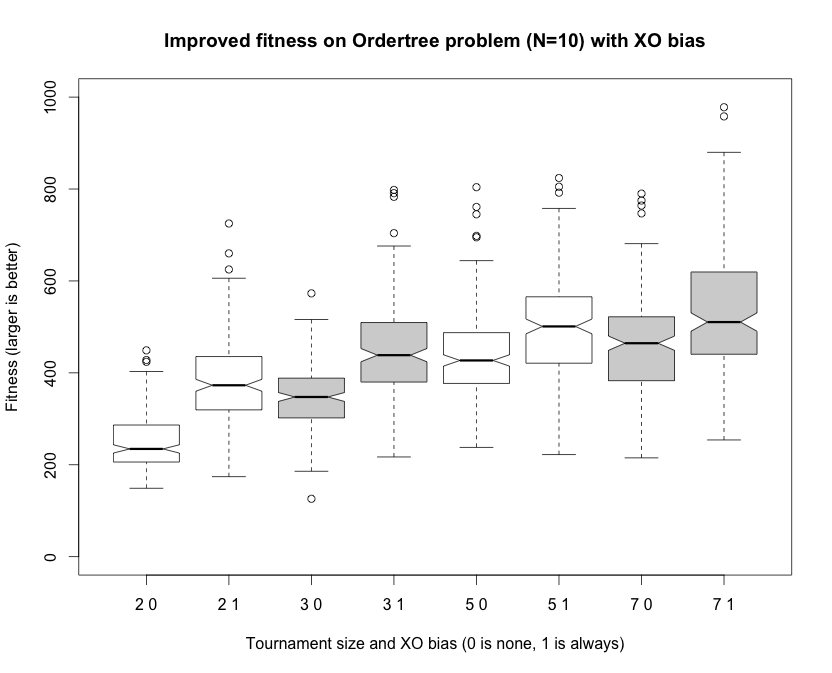
\includegraphics[width=0.45 \textwidth]{Plots/Ordertree_results.png}
\caption{Impact of crossover bias on fitness for Ordertree problem for various tournament sizes.}
\label{fig:Ordertree_results}
\end{figure}

\begin{figure}
\centering
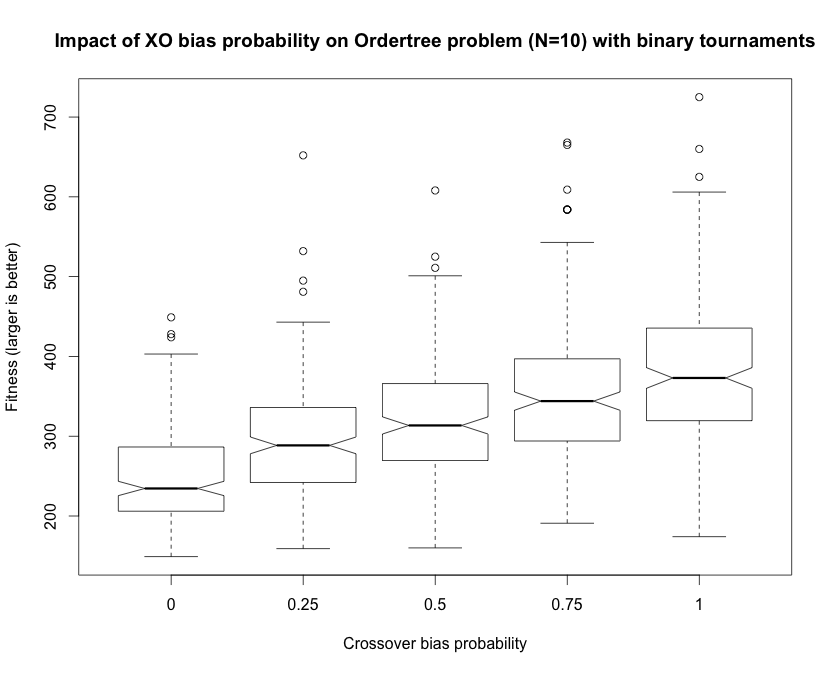
\includegraphics[width=0.45 \textwidth]{Plots/Ordertree_XO_bias_prob_binary_tournaments.png}
\caption{Impact of crossover bias on fitness for Ordertree problem for binary tournaments.}
\label{fig:Ordertree_results_binary_tournaments}
\end{figure}

\subsection{U.S. Change problem}

\begin{figure}
\centering
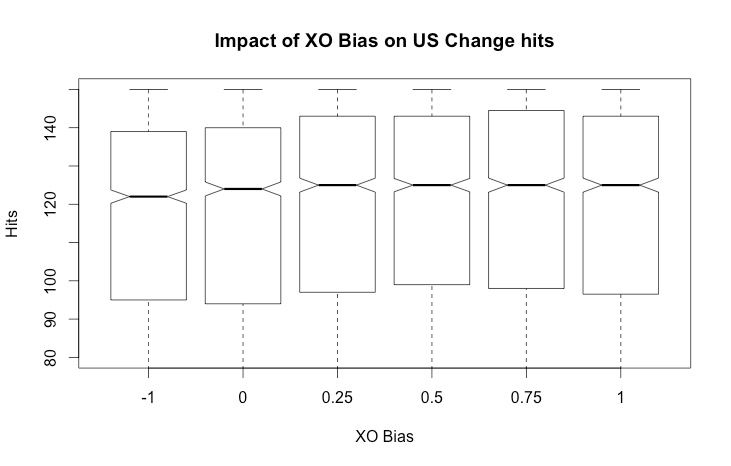
\includegraphics[width=0.45 \textwidth]{Plots/US_change_hits.png}
\caption{Impact of crossover bias on the number of hits for the US Change problem.}
\label{fig:USChange_Hits}
\end{figure}

\begin{figure}
\centering
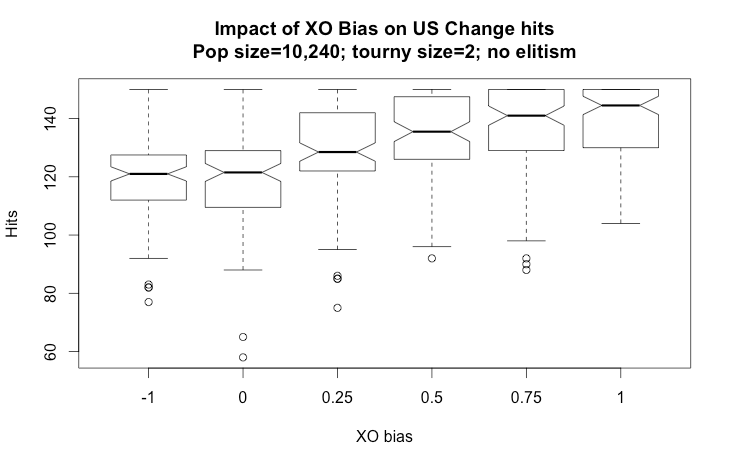
\includegraphics[width=0.45 \textwidth]{Plots/US_change_hits_tourny2_noElitism.png}
\caption{Impact of crossover bias on the number of hits for the US Change problem, limited to binary 
tournaments and no elitism.}
\label{fig:USChange_Hits_tourny2_noElitism}
\end{figure}

\begin{figure}
\centering
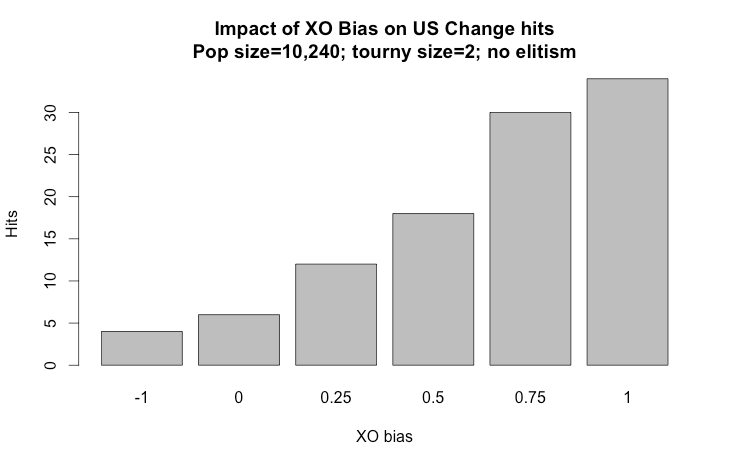
\includegraphics[width=0.45 \textwidth]{Plots/US_change_successes_tourny2_noElitism.png}
\caption{Impact of crossover bias on the number of successes runs for the US Change problem, limited to 
binary tournaments and no elitism.}
\label{fig:USChange_Successes}
\end{figure}


\begin{figure}
\centering
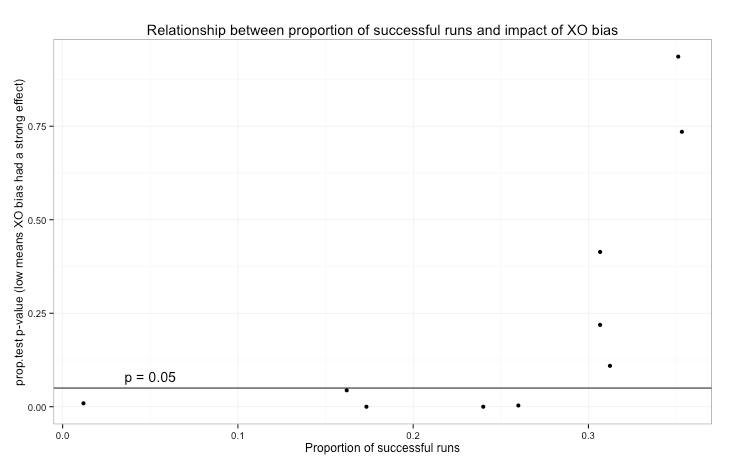
\includegraphics[width=0.45 \textwidth]{Plots/US_change_Bias_impact_vs_success.png}
\caption{Relationship between proportion of successful runs and the impact of crossover bias.}
\label{fig:USChangeBiasImpactVsSuccess}
\end{figure}

\subsection{Symbolic regression problems}

\subsubsection{Sine problem}

\begin{figure}
\centering
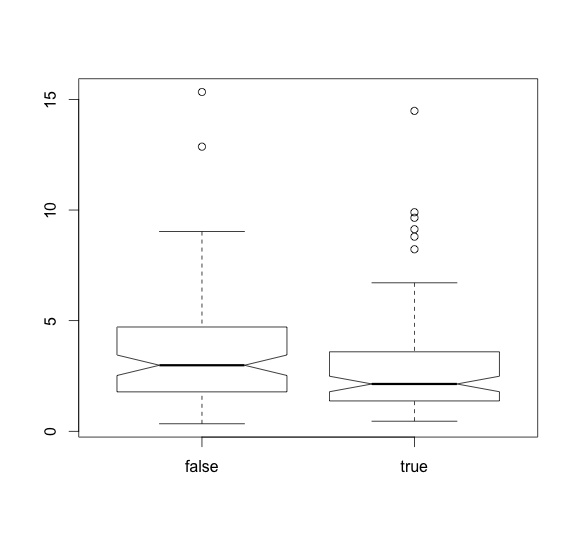
\includegraphics[width=0.45 \textwidth]{Plots/Sine_bias_results.png}
\caption{Impact of crossover bias on the sine symbolic regression problem}
\label{fig:sineBiasResults}
\end{figure}

\begin{figure}
\centering
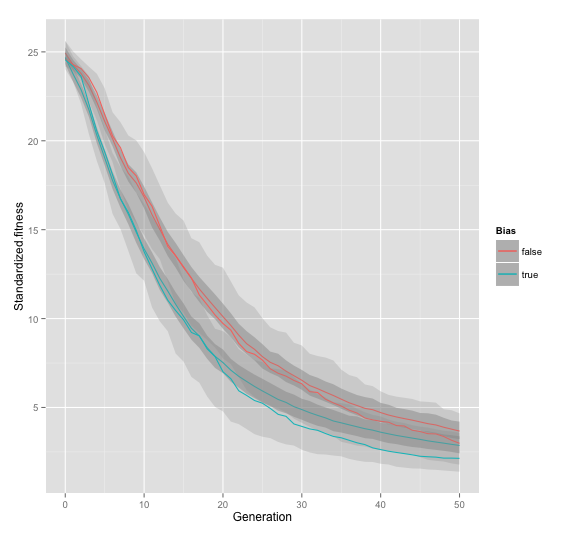
\includegraphics[width=0.45 \textwidth]{Plots/Sine_generations.png}
\caption{Impact of crossover bias on the fitness over time for the sine symbolic regression problem}
\label{fig:sineFitnessOverTime}
\end{figure}

\subsubsection{Pagie-1 problem}

\begin{figure}
\centering
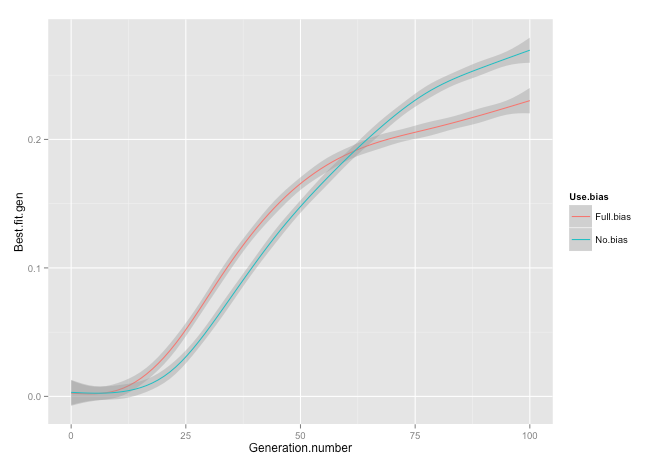
\includegraphics[width=0.45 \textwidth]{Plots/Pagie-1_fitness_vs_time.png}
\caption{Impact of crossover bias on the fitness over time for the Pagie-1 symbolic regression problem}
\label{fig:Pagie1FitnessOverTime}
\end{figure}

\begin{figure}
\centering
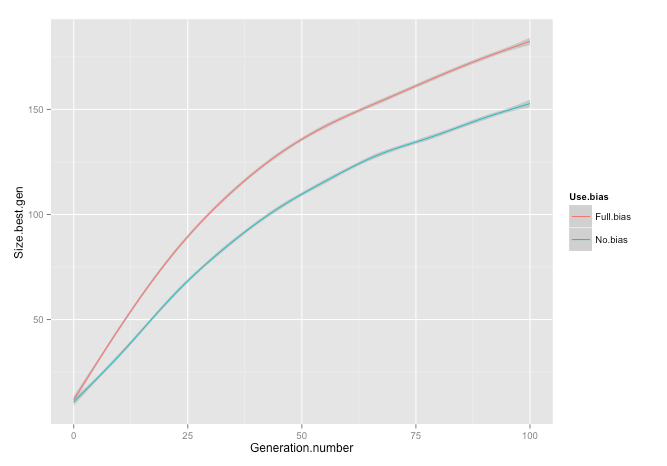
\includegraphics[width=0.45 \textwidth]{Plots/Pagie-1_size_vs_time.png}
\caption{Impact of crossover bias on the tree size over time for the Pagie-1 symbolic regression problem}
\label{fig:Pagie1SizeOverTime}
\end{figure}

\begin{figure}
\centering
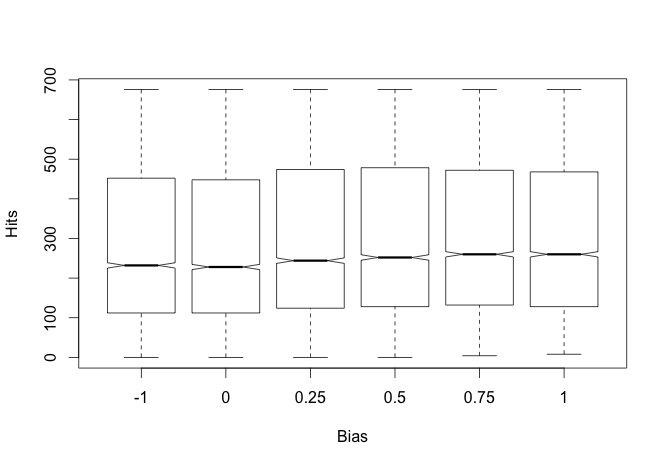
\includegraphics[width=0.45 \textwidth]{Plots/Pagie-1_Hits_vs_Bias.png}
\caption{Impact of crossover bias on the number of hits for the Pagie-1 symbolic regression problem. 
Unfortunately I'm not immediately sure what (sub)set of data this includes.}
\label{fig:Pagie1Hits}
\end{figure}

\begin{figure}
\centering
\includegraphics[width=0.45 \textwidth]{Plots/Pagie-1_Successes_vs_Bias.png}
\caption{Impact of crossover bias on the number of successes (runs that exactly solve the problem) for the 
Pagie-1 symbolic regression problem. Unfortunately I'm not immediately sure what (sub)set of data this 
includes.}
\label{fig:Pagie1Successes}
\end{figure}

\begin{figure}
\centering
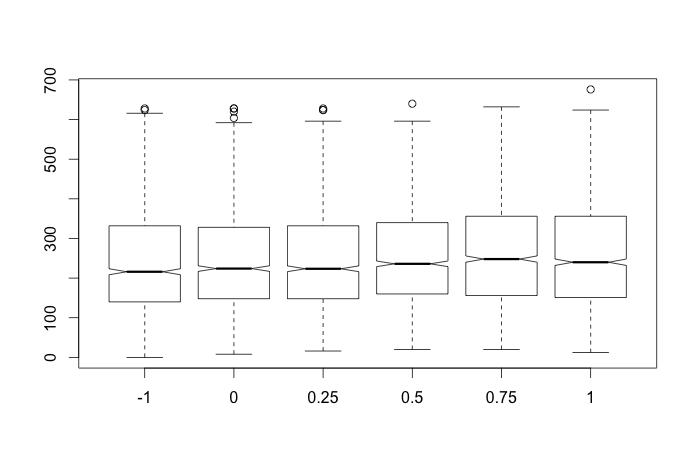
\includegraphics[width=0.45 \textwidth]{Plots/Pagie-1-koza2_no_Tarpeian.png}
\caption{Impact of crossover bias on the number of hits when using the koza2 function set for the Pagie-1 
symbolic regression problem.}
\label{fig:Pagie1Koza2}
\end{figure}

\begin{figure}
\centering
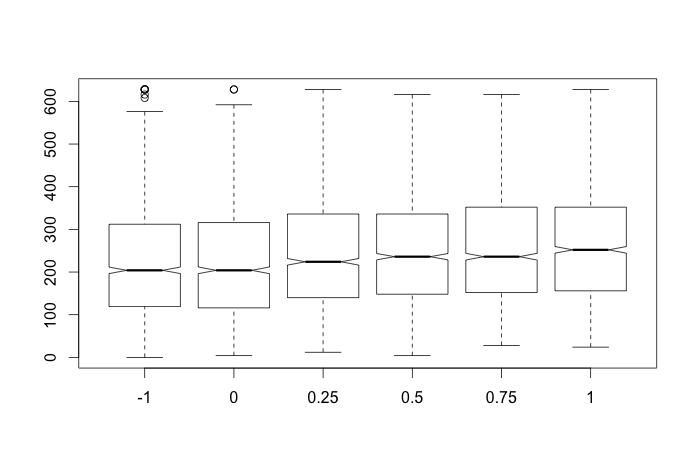
\includegraphics[width=0.45 \textwidth]{Plots/Pagie-1-tarp.png}
\caption{Impact of crossover bias on the number of hits when using the koza2 function set and Tarpeian bloat 
control for the Pagie-1 symbolic regression problem.}
\label{fig:Pagie1Koza2Tarpeian}
\end{figure}

\subsection{Santa Fe Trail problem}

I did a small-ish set of runs early on, so the setup for this isn't really the same as for the later problems. The 
only ``parameter sweep'' I did was XO bias on (i.e., 1) or off (i.e., 0). I only ran 50 generations, and the setting 
to stop early if a solution was found was turned on, so not all the runs went out to 50 generations. There were 
200 runs total, 100 with bias and 100 without.

\section{Conclusions} \label{Conclusions}

\section*{Acknowledgements}

\pagebreak

\bibliographystyle{acm}
\bibliography{Research_2015}

\end{document}